\documentclass[midd]{thesis}

\usepackage{graphicx}
\usepackage{times}
\usepackage{amsmath}
\usepackage{booktabs}
\usepackage[table,xcdraw]{xcolor}

\bibliographystyle{plain}


\title {Computational Aesthetic Evaluation using Convolutional Neural Networks}

\author {Teddy Knox}
\adviser {Professor Christopher Andrews}
% \conferralmonth {May}
% \conferralmonth {2015}

\begin{document}

\maketitle

\begin{abstract}
The accuracies of state-of-the-art machine learning techniques have exceeded the accuracy of humans at certain limited tasks, suggesting the computers will soon be able to complete many sophisticated tasks competently. This study tested the accuracy of state-of-the-art convolutional neural networks for modeling the statistically-defined visual aesthetic tastes of randomly generated triangle art. Our trained model demonstrated no predictive power at this task. Further research will be needed to interpret this result.
\end{abstract}

\begin{acknowledgements}
I dedicate this paper to science.
\end{acknowledgements}

\contentspage
\tablelistpage
\figurelistpage

\normalspacing \setcounter{page}{1} \pagenumbering{arabic}

\chapter{Introduction}
\label{sec:intro}

Machine learning is a broad discipline of computer science that has seen rapid advances in recent years, and has the potential to impact all human enterprises. The latest algorithms are capable of competitive or even better-than-human performance [citation needed] on certain tasks, and their applications are increasing in proportion to the availability of training data. One such application will be in the field of generative art and design. Generative art is art that is created procedurally, often with the help of a computer. Until recently, the use of co mputers in art and design has been limited to rote tasks such as preparing renderings and generating randomness, but advances in machine learning may soon enable computers to contribute higher-level aspects of the creative process, such as creative exploration and Computational Aesthetic Evaluation. Computation Aesthetic Evaluation (CAE) is the problem in generative art research of programming a computer to subjectively differentiate between aesthetically pleasing and displeasing content. This problem is important to the field of generative art for its potential to automate searches for aesthetic solutions, and would also be useful for building personalized recommendation systems. This research investigates the applicability of state-of-the-art general-purpose pattern recognition algorithms for Computational Aesthetic Evaluation. This experimentation is motivated by an interest in discovering the limits of these impressive models. By evaluating their accuracy on unconventional datasets of unknown complexity, we hope to gain a better understanding of both the model's capabilities and the hidden structure of the dataset. This paper first provides background and formulates the problem, then explains the experimentation in detail, and concludes with a discussion of results and future uses of machine learning models for the analysis of artistic content.

% general introduction to CAE and generative art
% why we would care? vision
% WHat is this particular thesis about -> applying ml to the problem
% what are we doing? -> convolutional neural network
% more specific -> ran a study, using GoogLeNet
% What we will discuss ->

Accurate Computational Aesthetic Evaluation algorithms would be useful in the fields of generative art and recommendation systems. The scale and quality of generative art would increase quickly if computers were capable of contributing to creative decision making and aesthetic evaluation inherent in the creative process. Despite their enormous computational power, the primary use of modern computers in generative art falls into the category of rendering procedures into their realized form, rather than participating in the search for aesthetic beauty. Advances in machine learning for pattern recognition have proved useful in many different types of well-defined tasks. In this study we apply modern image classification techniques using convolutional neural networks to the problem of computational aesthetic evaluation, observing whether they are capable of learning the tastes evident in a dataset of randomly generated triangle art, labeled with aesthetic quality ratings.

Convolutional Neural Networks (CNNs) are a type of model inspired by the biology of the human visual processing center, and have been shown to be the most effective model for image recognition to date.
% TODO: Cite this assertion
CNNs are a type of feed-forward artificial neural network architecture formed by layers of convolutional filters, trained to derive high-level features from low-level pixel data. These high-level features are powerful and versatitle data separators which are then typically fed into a non-linear classifier or regressor to produce final predictions. The network's parameters are learned through an iterative training process, where batches of examples are fed into the network and network parameters are adjusted to reduce prediction errors. Iterations of adjustments are made until the network's prediction accuracy on its training data converges or surpasses a threshold.

\chapter{Background}
Before examining this study we will explain background principles in the fields of Computational Aesthetics and Image Recognition.

\section{Related Work in Computational Aesthetics}
Computational aesthetics is a fledgeling interdisciplinary field formed by the overlap of research in machine learning, neuroethetics, and evolutionary psychology. Efforts in this field are mostly explorational, and few concrete advances have been made. The most cited papers in the field of Computational Aesthetics include ``Computational aesthetic evaluation: Past and future'', ``Defining computational aesthetics'', and ``Experiments in computational aesthetics''. These studies fall into practical and theoretical categories, roughly corresponding to top-down and bottom-up research strategies. Practical studies are oriented around conducting experiments to verify the correlation of commonly-held art school heuristics with subjective aesthetic ratings, in an effort make generalizations. Theoretical studies aim to develop a connectionist model for understanding aesthetics by drawing upon the insights of machine learning and neuroaethetics \cite{galanter2012computational, hoenig2005defining, machado2008experiments}.

% TODO: Talk about top-down work

The bottom-up work in computational aesthetics aims to develop an enlightened philosophical framework for understanding the human aesthetic system, and is indispensible for thinking clearly about bottom-up experimental work. Galanter and Hoenig grapple head-on with the field's conceptual entanglement, with an awareness of the ``baby steps'' that any progress will look like. We suspect, and we think these researchers would agree, that generalizable advances in this field will be deeply related to machine learning and neuroesthetics (the biological study of aesthetics), rather than more practical areas of aesthetics offering guidelines like the Gestalt laws. Given that philosophers have been devising high-level heuristics for judging aesthetics since antiquity, it seems unlikely that the increased availability of computational power will directly impact our conception of the problem.

To provide context, we will briefly summarize the history and foundational ideas of computational aesthetics.

One of the most significant advances in the greater philosophy of aesthetics is owed to Mathematician G.D. Birkoff, who spent a year traveling the world to study beauty across cultures, before proposing a speculative psychological model for quantifying it. In his oft-referenced 1933 paper \emph{Aesthetic Measure}, Birkoff proposes that the perception of beauty is the pleasurable resolution of apparent complexity of a stimulus into a compact mental representation. He codified this relationship into a formula that relates degree of beauty $B$ to the balanced ratio of order $O$ to complexity $C$.

\begin{align*}
B &= \frac{O}{C}
\end{align*}

The plausibility of Birkoff's measure as a guiding philosophy of aesthetics earned it significant attention in later experimental studies. The recent work of Ragau et. al. and Koshel et. al. draws from information theory to approximate the parameters of Birkoff's formula. They used zeroth-order measures such as Kolmogorov complexity and Shannon entropy \cite{rigau-1, koshelev-1}, to demonstrate encouraging correlations between Birkoff's measure and human-rated beauty.

These results are significant enough to validate the direction Birkoff's core idea --- that the human aesthetic response is tuned to respond to stimuli that are sophisticated yet digestible. Novel ideas in the fields of machine learning, neuroesthetics, and the emerging field of evolutionary philosophy (The top-down study of evolutionary adaptations), may be a way forward.
% TODO: rework the following
Philip Galanter stands at the intersection of these fields, and subscribes to the view that humans find stimuli with the greatest ``effective complexity'' to be the most engaging, and thus the most rewarding. Within this framework, the problem of computational aesthetics can be expressed as the study of how humans judge ``effective complexity'' \cite{galanter-1,galanter-2,galanter-3,galanter-4}. Effective complexity is a theoretical measure conceived by Gell-Man et. al. \cite{gell2004effective} to roughly correspond to the colloquial meaning of the word ``complex''. Effective complexity measures resistance to entropic forces rather than resistance to signal compression. For example, a symphony by Mozart possesses greater effective complexity than white noise, because it presents a manageable amount of harmonious sophistication for us to process.

\begin{figure}
\centering
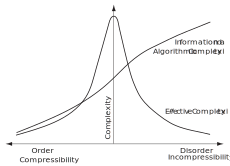
\includegraphics[width=0.75\textwidth]{figures/effectivecomplexity.pdf}
\caption{Relationship between effective complexity and order}
\label{fig:effectivecomplexity}
\end{figure}

In seeking to develop a computational aesthetic evaluator this research is touching onto topics of information complexity and effective complexity, as developed by these researchers. These improving measures will likely align closely with the neurology of human sensory perception. It may already be possible to draw parallels between the principles underlying machine learning systems and Birkoff's measure, since the success of these systems already depend on learning of compact, high-level represenations of low-level inputs. This is one of the reasons we became interested in applying the latest advances in image recognition to the field of computational aesthetics. Convolutional neural networks are models inspired by the structure of the human visual cortex, and as such may have a higher chance of making accurate predictions.

Several types of machine learning techniques have been used in computational aesthetic evaluation algorithms with increasing success.

Penousal Machado et al \cite{machado2008experiments} implemented an iterative artificial artist system by combining a neural network with an evolutionary programming system. The neural network served as an aesthetic evaluator, and was trained on manually extracted features for every step of the iteration. The genetic programming system would generate populations of artwork, using the aesthetic evaluator as its fitness function. In observing the creative process as alternation between creative and evaluative stages, their system repeatedly produces populations of ``drafts'' and then evaluates how well they match a constant set of target images. The target images they chose were pieces of artwork. The drafts that most closely matched the target images would then seed the next generation of drafts, and the aesthetic evaluator would be retrained to recognize all of the drafts as non-target images. This feedback loop was designed to ensure that every generation of drafts would be different from the last, and hopefully resulting in greater image complexity. The entire algorithm produces interesting results until the 12th generation, when classification error increases steeply.

The system's aesthetic evaluator uses 41 features based metrics like fractal complexity and zipf distribution, each applied over a variety of image channels such as hue or saturation. Although these features provided some predictive value, none were discovered to be orders of magnitude more predictive than the others. Even as more evolved drafts are added to the non-target training set, the classifier consistently trains to more than 99\% accuracy. In other words, the classifier is consistently good at separating images of paintings and computer generated images of previous generations, but grows worse at predicting the class of future generations as iterations progress. This experiment demonstrates how neural networks are being applied in novel ways to explore computer capabilities for generating and recognizing aesthetically pleasing art. % maybe cut this out?

Many have also put genetic algorithms to the task of coming up with novel solutions to design problems, and have incorporated aesthetic features into their fitness function by manually extracting heuristics of good design as features for some sort of classifier. These approaches demonstrate acceptable results, and are generally limited by their set of handmade low-level features for prediction. % citations??

% Include section on Melbourne study using Self Organizing Maps?

\section{Related Work in Image Classification}

Machine learning presents some of the most promising opportunities for advances in computational aesthetics. The accuracy of state-of-the-art pattern recognizers have been increasing steadily from year to year since the mid-2000s. Researchers think that these encouraging advances in data science have been the result of a combination of the increasing availability of huge datasets, the decreasing cost of computation, and the influx of new ideas and interest \cite{szegedy2014going}.

Of particular interest to me was a powerful image recognition architecture that Google developed to win the 2014 Imagenet Large Scale Visual Recognition Challenge (ILSVRC)  \cite{szegedy2014going}. ILSVRC 2014 challenged participants to correctly classify a set of test images derived from 1000 different Imagenet categories. Some of the categories look extremely similar, and demanding a near human level of recognition ability to differentiate. For example, the Siberian huskey and the Eskimo dog look very similar, and both were included as categories for the Imagenet challenge. With an appreciation of the ability of GoogLeNet to recognize patterns, we wondered if this same architecture could demonstrate a similar level of ability at aesthetic evaluation tasks.

% The CNN training process is computationally intentensive, requiring training time that grows quickly with the width and depth of layers. The main model we used for classification is a replica of the Google Research entry into the 2014 Imagenet Large-Scale Visual Recognition Challenge (ILSVRC 2014), dubbed GoogLeNet. Imagenet is an image database organized according to the wordnet hierarchy, and the ILSVRC 2014 challenge tested the ability of models to accurately tag photos with up to 5 tags out of a body of 1000. The GoogLeNet architecture won the ILSVRC challenge in 2014, achieving an impressive top-5 error rate of 6.67\%. GoogLeNet is an extremely deep network comprised of 24 layers, [how many convolutional layers?], and operates with [how many parameters?]. A full discussion of the qualities and mechanics of convolutional neural networks will come in the theory section.

\chapter{Design}

% Deeper discussion on color theory generalizations.

% \section{Generative Art}

Three motivations informed the design of this experiment.

The first was an interest in whether convolutional neural networks might prove more effective than hand-programmed feature extraction techniques for computational aesthetic evaluation. In our literature review we noticed that a majority of experiments in aesthetic evaluation rely on tens of hand-programmed feature extractors and standard machine learning classifiers to produce modest results. These approaches are based on rigid assumptions on the appearance of aesthetic value. One of these experiment extracted a feature corresponding to the dynamic contrast of colors in the image, and another corresponding to the diversity of colors in a patch of an image. Using a bunch of hand-programmed feature extractors in these experiments may be an efficient way to try to discover an ultra-effective feature extractor, but if this search is not fruitful it may make sense to turn towards more versatile feature extraction techniques. In the task of image recognition, convolutional neural networks are effective for recognizing extremely different patterns; could a CNN do for aesthetic evaluation what it did for image recognition?

The second motivation informing the design of this study was an interest in the separability of subjective aesthetic judgements of arbitrary complexity. We wanted to throw a dataset of unknown difficulty at our model and see what it would give me back. There is much hype surrounding the capabilities of this type of model, some of which we had admittedly bought into. In an effort to challenge ourexpectations of these models, we asked whether such a model could remain effective on a type dataset it was not designed for.

The third motivation was an interest in the relationship between the accuracy of our classifier for a given image and the type of image provided to the classifier. If we used a simple type of art for our experiment, it might be easier to identify pattern or types of images that the classifier finds it difficult to classify.

With these factors in mind, we designed an experiment. The body of artwork for rating would be randomly generated triangle art. We would build a training interface for rating these images, where we would assign each presented image a completely subjective binary rating of attractiveness. We would click the green button if an image looked good to me, and the red button if it did not. In order to ensure the internal consistency of ourratings, we would make sure to give each image more than one rating during the training proces. We represented a ``thumbs up'' rating with a 1, and a ``thumbs down'' rating with a 0. If an image received conflicting ratings, its recorded label would become 0, to avoid introducing controversial images to our classifier. With a dataset of consistently rated images, we would train GoogLeNet on a big portion of the data, and test GoogLeNet on the rest.

To perform this experiment we would need to assemble a relatively small dataset of images with ratings using a training interface, and we would need an instance of the GoogLeNet classifier.

% \section{Compuational Aesthetic Evaluation - Convolutional Neural Network}
%
% We used a single CNN models that come with Caffe ``out of the box'' to test their efficacy, rather than attempt to customize a model to this task. The first model we tested is called GoogLeNet, which won the ImageNet Large Scale Visual Recognition Challenge in 2014.

\chapter{Implementation}


\section{Training Interface}

Assembling a dataset was relatively straightforward. We built an interface for generating images and recording their user ratings using python and web technologies. After each rating submission, the interface would algorithmically decide which image to show next. We programmed it randomly alternate between new images and existing images, with a bias towards rating those existing images with the fewest ratings.
% TODO: Flagged for removal
For fun and convenience we added swipe gesture support to the mobile interface, allowing for rating on-the-go.

The algorithm for generating each image worked as follows. First a blank 256x256 canvas would be filled with a random color. Then a random number of triangles (2-6) would be drawn on top of each other. Triangles' corners would be randomly placed, and their fill color would be random. All of the randomness used was uniform, and all of the colors were specified in HSL format, so that the lightness of each randomly selected color could be restricted to an attractive range of values.

Over the course of a few days we made roughly 4000 ratings on  2000 images. In rating triangle art for several hours we was surprised by how quickly we would grow tired of judging the images. In computational aesthetic literature user fatigue is a recognized difficulty with interactive training systems, as it dramatically limits the scale of data collection. In order to reach 4000 high-quality ratings, we found it useful to take breaks every 10 minutes, and try not to adjust ourtaste in the triangle images. We decided to make 4000 ratings rather unscientifically. At this stage in the experiment we was anxious to begin classifying ourdata, and unsure of whether a dataset of, say, 10,000 example would be significantly better than a dataset of 4,000 examples. Our intuition, based on the published results of companies using large datasets, was that unless we could produce at least an order of magnitude more training examples, our result's accuracy would not vary by much. We labeled 75\% of the images with low aesthetic value and the remaining 25\% with high aesthetic value.

% sigmoid graph of data quantity by model accuracy

% relevant https://xkcd.com/915/
\section{Classifier}

We decided to use a popular neural network framework called ``Caffe'' to implement our classifer. Caffe began at the Berkeley Language and Vision Center in 2013, and offers a well-designed and efficient interface for designing, training, and running neural networks. Caffe comes packaged with several example model specifications, one of which thoroughly describes an untrained replica of GoogLeNet. Using this specification of GoogLeNet ensured the accuracy of our model, and was conveniently saved us time.

Training convolutional neural networks is notoriously computationally intensive. To model our data in a resonable amount of time, we ended up renting an AWS g2.2xlarge instance, complete with a graphics card sporting 1,536 CUDA cores. This allowed for us to take advantage of enticing GPU speedups that Caffe optionally offers.
% TODO: CPU VS GPU graphic
This cloud setup was convenient both financial and technically. Amazon's pay-as-you-go billing model meant we only paid for computing hours that we used, and their transparent cloud imaging technology meant that our Caffe installation would persist after restarts.
% TODO: Flagged for removal
\footnote{As an aside, instant remote access to high-powered computing is a magical experience.}

Next we retrofitted the GoogLeNet architecture included in Caffe to output predictions for 2 labels, instead of 1000, and began our experiment. To ensure test accuracy, our classifier used a 10-folds cross validation scheme, in combination with careful.

\chapter{Results}

% TODO: Write this section

% introduce experiment.

% data analysis
  % how many ratings
  % how many images
  % rating stddev
% model description
  % how long did the model take to train
  % effective hyperparameters
    % SGD, gamma 0.6, step size 100, test often
% plot of avg training loss + avg test loss vs iterations

\begin{table}[h]
\centering
\resizebox{\textwidth}{!}{%
\begin{tabular}{@{}rlllllllllllll@{}}
\toprule
\textbf{k-Fold} & \multicolumn{10}{c}{\textbf{Training Iteration}} & \textbf{\begin{tabular}[c]{@{}l@{}}Best \\ Accuracy\end{tabular}} & \textbf{\begin{tabular}[c]{@{}l@{}}Null\\ Hypothesis\\ Accuracy\end{tabular}} & \textbf{\begin{tabular}[c]{@{}l@{}}Accuracy\\ Above \\ Null\end{tabular}} \\ \midrule
\textbf{} & 100 & 200 & 300 & 400 & 500 & 600 & 700 & 800 & 900 & 1000 &  &  &  \\ \midrule
\multicolumn{1}{r|}{1} & 0.758 & 0.766 & 0.756 & 0.766 & \textbf{0.781} & 0.768 & 0.773 & 0.770 & 0.770 & \multicolumn{1}{l|}{0.773} & 0.781 & 0.765 & 0.016 \\
\multicolumn{1}{r|}{2} & 0.705 & 0.699 & 0.715 & 0.715 & 0.732 & 0.727 & \textbf{0.746} & 0.734 & 0.732 & \multicolumn{1}{l|}{0.707} & 0.746 & 0.738 & 0.027 \\
\multicolumn{1}{r|}{3} & 0.754 & 0.765 & 0.758 & \textbf{0.803} & 0.748 & 0.691 & 0.752 & 0.682 & 0.767 & \multicolumn{1}{l|}{0.723} & 0.803 & 0.761 & 0.042 \\
\multicolumn{1}{r|}{4} & 0.752 & 0.752 & \textbf{0.770} & 0.762 & 0.738 & 0.75 & 0.760 & 0.756 & 0.752 & \multicolumn{1}{l|}{0.756} & 0.770 & 0.755 & 0.014 \\
\multicolumn{1}{r|}{5} & 0.695 & 0.707 & 0.676 & 0.707 & 0.682 & 0.709 & 0.697 & \textbf{0.713} & 0.709 & \multicolumn{1}{l|}{0.699} & 0.713 & 0.699 & 0.014 \\
\multicolumn{1}{r|}{6} & 0.709 & 0.713 & 0.736 & 0.707 & 0.725 & 0.699 & 0.738 & \textbf{0.748} & 0.734 & \multicolumn{1}{l|}{0.713} & 0.748 & 0.713 & 0.035 \\
\multicolumn{1}{r|}{7} & 0.699 & 0.699 & \textbf{0.752} & 0.723 & 0.699 & 0.729 & 0.699 & 0.727 & 0.717 & \multicolumn{1}{l|}{0.707} & 0.752 & 0.700 & 0.052 \\
\multicolumn{1}{r|}{8} & 0.764 & 0.760 & 0.766 & 0.758 & 0.768 & 0.773 & 0.766 & 0.750 & 0.758 & \multicolumn{1}{l|}{\textbf{0.797}} & 0.797 & 0.757 & 0.039 \\
\multicolumn{1}{r|}{9} & 0.703 & 0.715 & 0.658 & 0.707 & 0.684 & \textbf{0.714} & 0.713 & 0.705 & 0.709 & \multicolumn{1}{l|}{0.697} & 0.714 & 0.699 & 0.016 \\
\multicolumn{1}{r|}{10} & 0.740 & 0.748 & 0.742 & 0.729 & 0.736 & 0.752 & \textbf{0.766} & 0.760 & 0.727 & \multicolumn{1}{l|}{0.764} & 0.766 & 0.738 & 0.027 \\ \midrule
\multicolumn{1}{l}{\textbf{}} &  &  &  &  &  &  &  & \multicolumn{3}{r|}{\textbf{Average}} & 0.759 & 0.733 & 0.029 \\ \bottomrule
\end{tabular}
}
\caption{GoogLeNet test accuracy across 10-fold cross-validation and compared with null hypothesis priors}
\label{my-label}
\end{table}

\chapter{Discussion of Results}

% TODO: write this section

% with dataset of this size model trains to optimal test accuracy very quickly, takes longer to overfit

The outcome of this experiment was a classifier which demonstrated no predictive power on the dataset provided. Normally this would be a


\chapter{Conclusion}

% TODO: Write this section

% this is meta-recognition
% we're not asking what this is, were asking whether what this is looks good.

% address each of the motivations

% too many motivations?

% this dataset is different from imagenet in that for imagenet, when asked to classify an image of a bear

Given the difficulty of defining art itself, it is no surprise that the criticism and reception of art itself is as nebulous. Yet despite the unclear underpinnings of aesthetic tastes, it is clear that aesthetic judgements are an integral part of everyday life. Short of machine intelligence, computerized judgements of aesthetics will likely never supercede our own, but in combination with our own, there is the potential for computers to make artists out of us all, or at least reduce the cost of aesthetically pleasing design.

The outcome of this experiment may not be clear and but the field of computational aesthetic evaluation will only gain in relevance as we strive to make our world more beautiful.

\nocite{*}
\bibliography{thesis}
\end{document}
